\begin{frame}{Hardware - Raspberry Pi 2}
  \begin{center}
    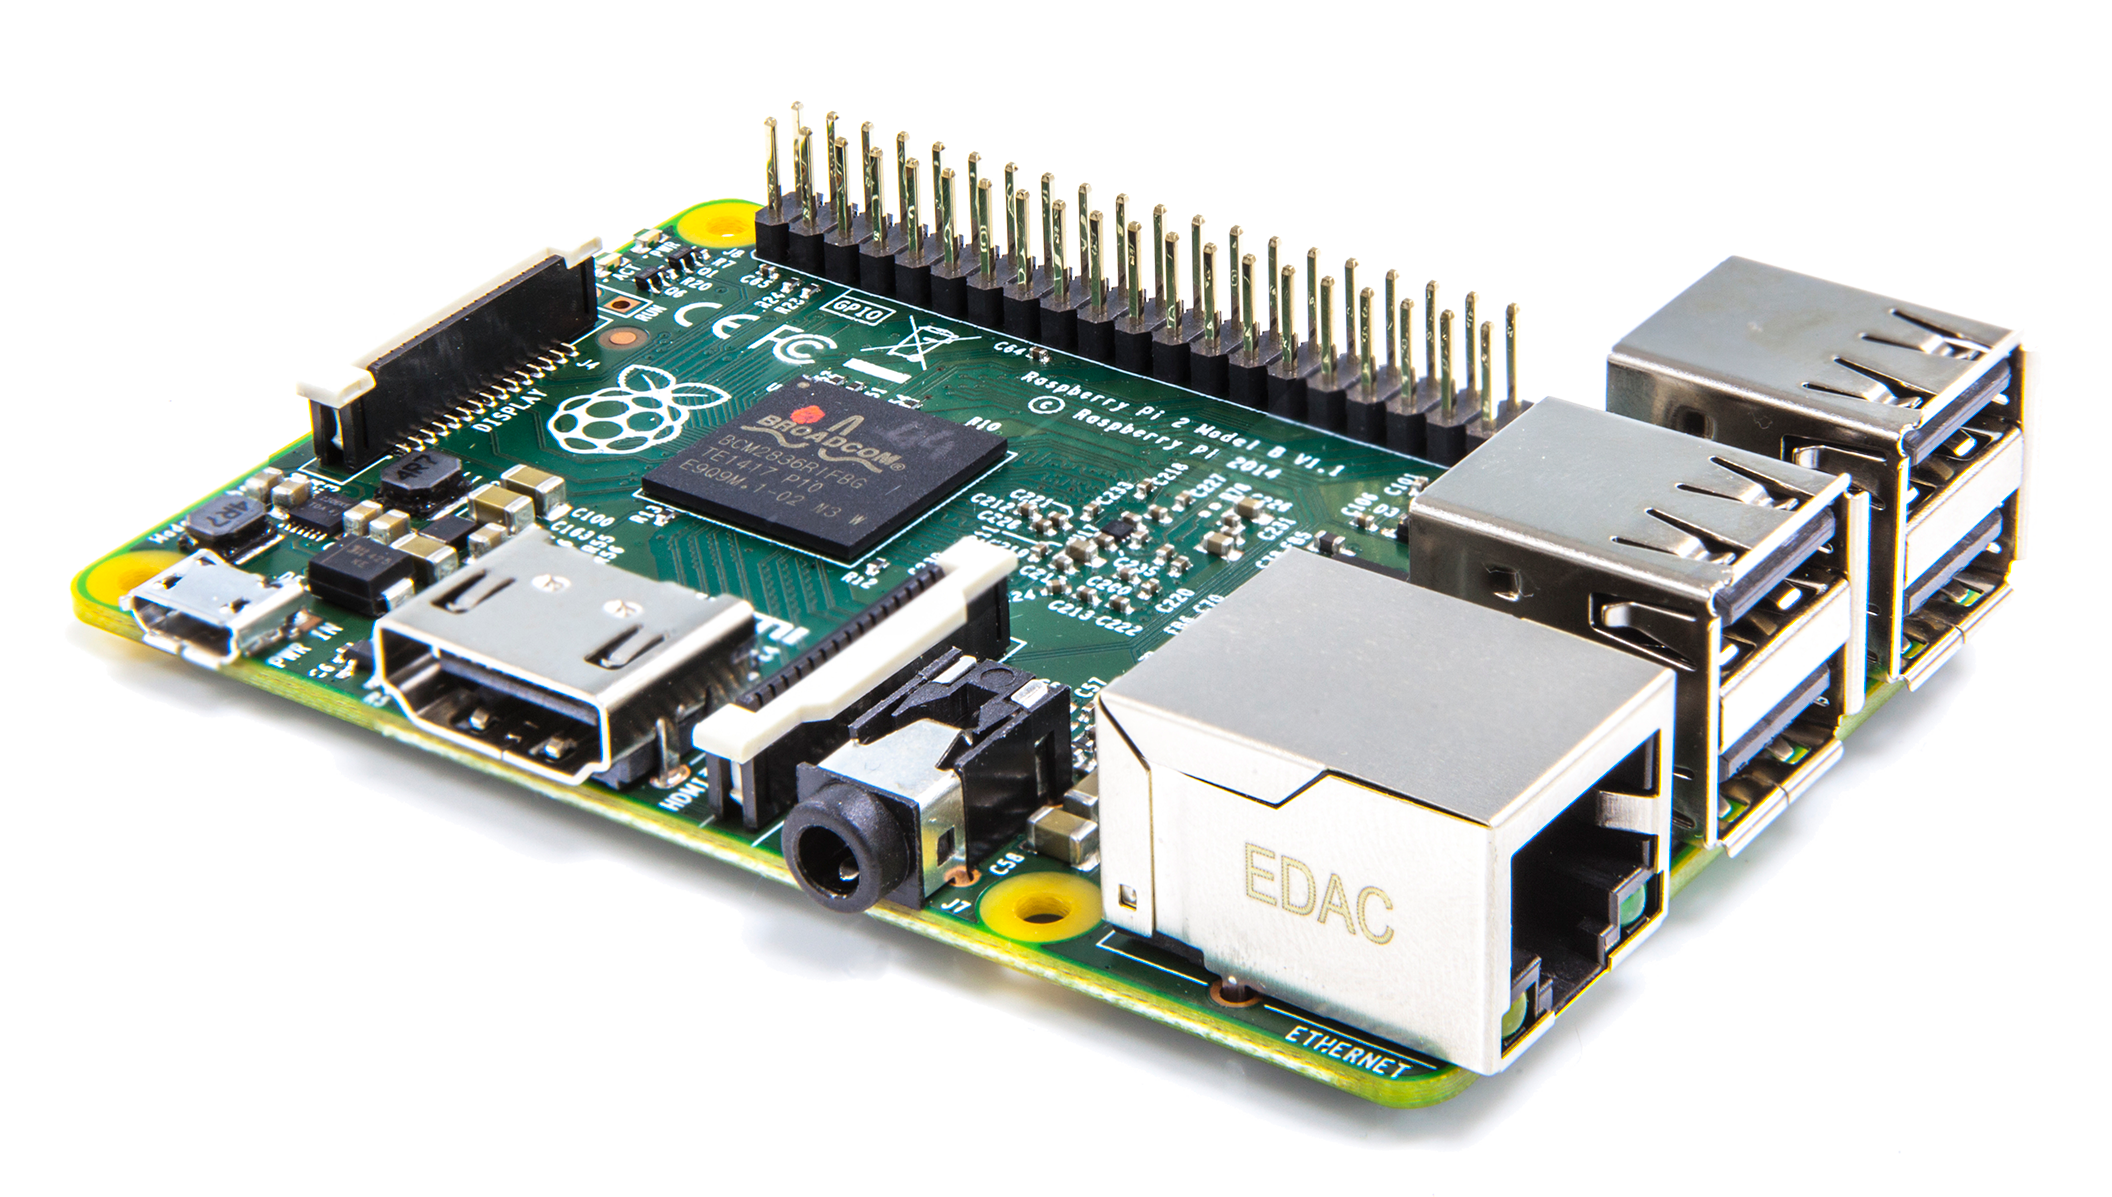
\includegraphics[width=\textwidth]{images/rpi2}
    \label{fig:rpi}
  \end{center}
\end{frame}

\begin{frame}{Hardware - Raspberry Pi 2 - Gründe}
  \Large
  \begin{itemize}
    \item Universell einsetzbar
    \item Sehr gutes Preis/Leistungs-Verhältnis
    \item Umfangreicher Support durch Community
    \item Große Basis unterstützter Software
    \item Einfach in der Handhabung
  \end{itemize}
\end{frame}

\begin{frame}{Hardware - Raspberry Pi 2 - Spezifikationen}
  \Large
  \center{
  \begin{tabular}{ l r }
    CPU & \texttt{ARM Cortex-A7}\\
    CPU-Kerne & \texttt{4}\\
    CPU-Takt & \texttt{900 MHz}\\
    RAM & \texttt{1 GB}\\
    \\
    Stromverbrauch & \texttt{max. 4 W} \\
    Preis & \texttt{\textasciitilde 40€}
  \end{tabular}}

\end{frame}

\begin{frame}{Hardware - RaspBee}
  \begin{center}
    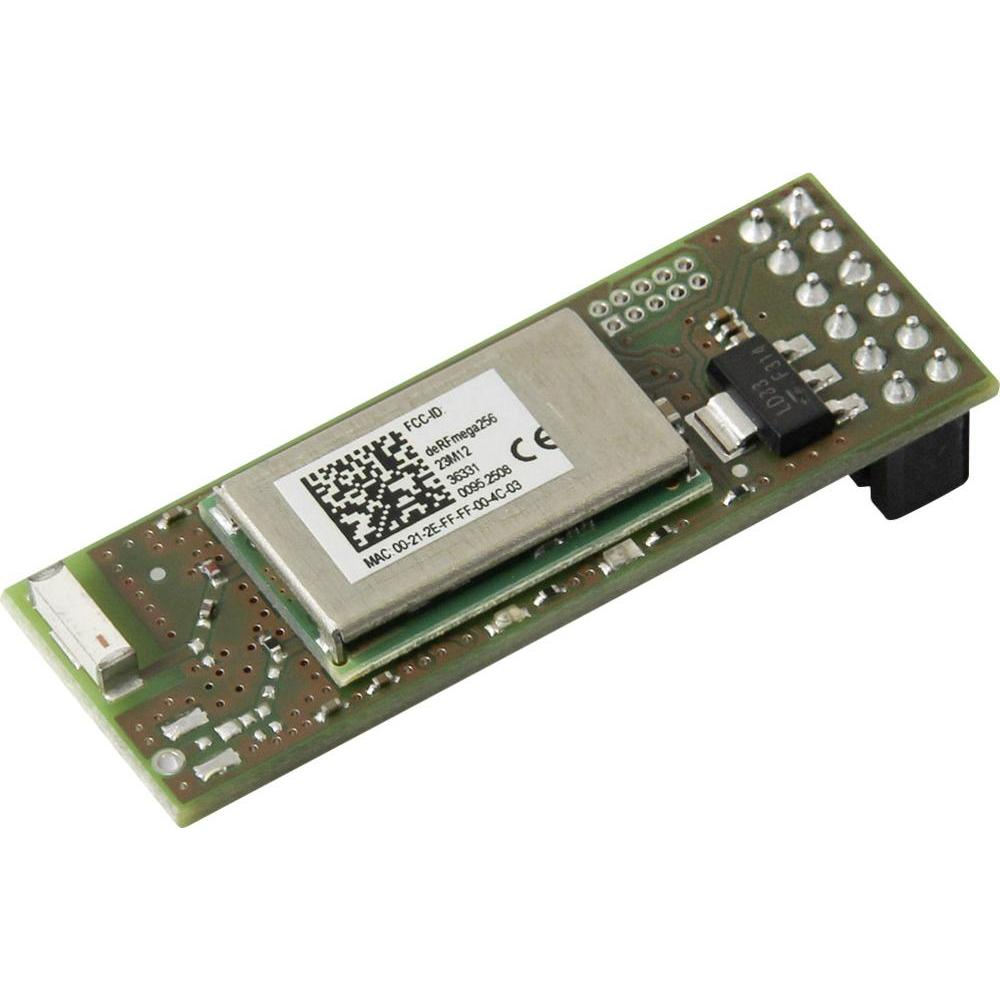
\includegraphics[width=\textwidth]{images/raspbee}
    \label{fig:rbee}
  \end{center}
\end{frame}

\begin{frame}{Hardware - RaspBee - Gründe}
  \Large
  \begin{itemize}
    \item Sehr gute Unterstützung für RPIs
    \item Komplette Verwaltungssoftware
    \item Gute Verfügbarkeit
    \item Weit verbreitet
  \end{itemize}
\end{frame}

\begin{frame}{Hardware - Hue}
  \begin{center}
    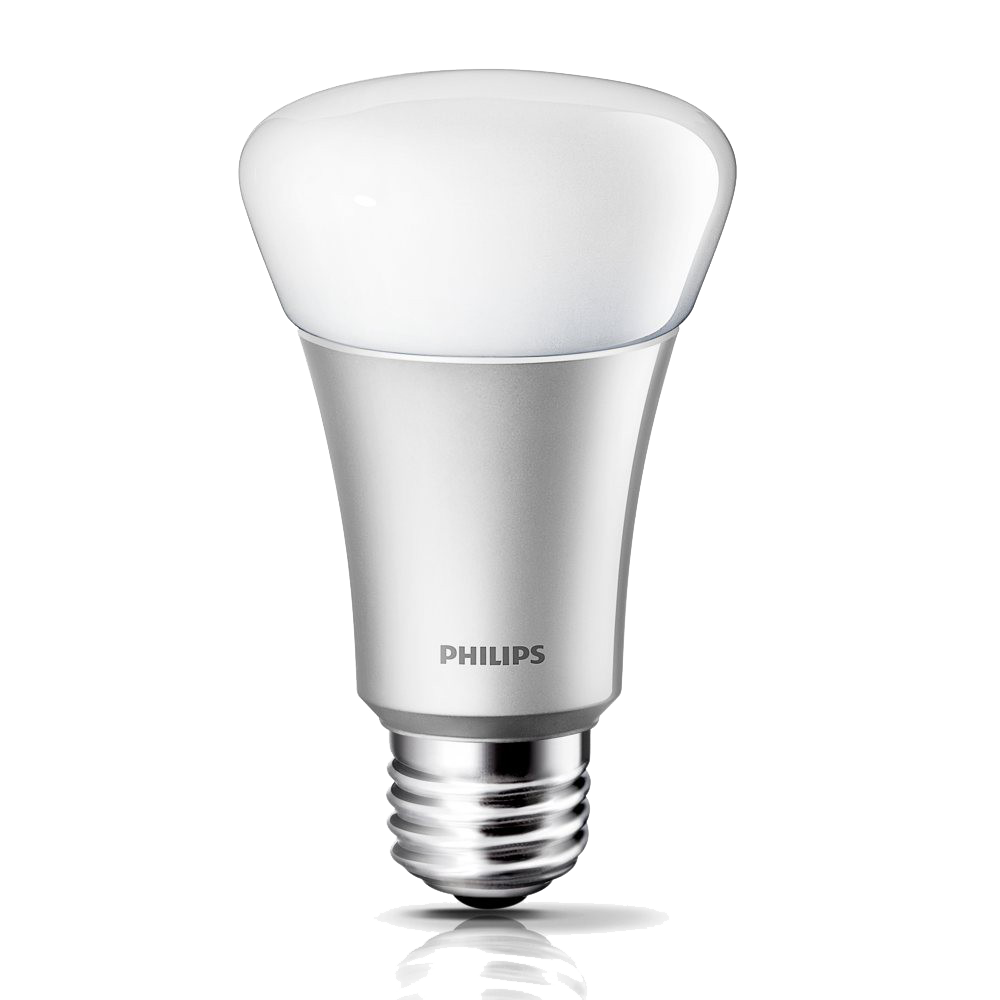
\includegraphics[width=0.7\textwidth]{images/hue}
    \label{fig:hue}
  \end{center}
\end{frame}

\begin{frame}{Hardware - Hue - Gründe}
  \Large
  \begin{itemize}
    \item Weite Verbreitung
    \item Gute Erfahrungen
    \item Gute Qualität
  \end{itemize}
\end{frame}

\begin{frame}{Hardware - Hue - Organisation}
  \Large
  \centering
  \begin{tikzpicture}
    % Lichter
    \draw [fill=red, draw=none] (-1.5,0) circle (0.3cm) node (hue1) {};
    \draw [fill=green, draw=none] (0,0) circle (0.3cm) node (hue2) {};
    \draw [fill=blue, draw=none] (1.5,0) circle (0.3cm) node (hue3) {};
    \draw [fill=yellow, draw=none] (4,0) circle (0.3cm) node (hue4) {};
    % Label für Lichter
    \node (hue1label) [above=0.3 of hue1]{Hue1};
    \node (hue2label) [above=0.3 of hue2]{Hue2};
    \node (hue3label) [above=0.3 of hue3]{Hue3};
    \node (hue4label) [above=0.3 of hue4]{Hue4};
    % Gruppen und Szenen
    \draw [draw=black, ultra thick] (0,0) ellipse (3.0cm and 1.8cm) node (group) {};
    \draw [draw=teal, ultra thick] (0.75,0) ellipse (1.5cm and 0.5cm) node (scene) {};
    % Label für Gruppen und Szenen
    \node (grouplabel) [above=1.5 of group]{Gruppe};
    \node (scenelabel) [below=0.3 of scene]{Szene};
  \end{tikzpicture}
\end{frame}
